\documentclass[noauthor,nooutcomes,12pt,hints,handout]{ximera}

\graphicspath{  
{./}
{./whoAreYou/}
{./drawingWithTheTurtle/}
{./bisectionMethod/}
{./circles/}
{./anglesAndRightTriangles/}
{./lawOfSines/}
{./lawOfCosines/}
{./plotter/}
{./staircases/}
{./pitch/}
{./qualityControl/}
{./symmetry/}
{./nGonBlock/}
}


%% page layout
\usepackage[cm,headings]{fullpage}
\raggedright
\setlength\headheight{13.6pt}


%% fonts
\usepackage{euler}

\usepackage{FiraMono}
\renewcommand\familydefault{\ttdefault} 
\usepackage[defaultmathsizes]{mathastext}
\usepackage[htt]{hyphenat}

\usepackage[T1]{fontenc}
\usepackage[scaled=1]{FiraSans}

%\usepackage{wedn}
\usepackage{pbsi} %% Answer font


\usepackage{cancel} %% strike through in pitch/pitch.tex


%% \usepackage{ulem} %% 
%% \renewcommand{\ULthickness}{2pt}% changes underline thickness

\tikzset{>=stealth}

\usepackage{adjustbox}

\setcounter{titlenumber}{-1}

%% journal style
\makeatletter
\newcommand\journalstyle{%
  \def\activitystyle{activity-chapter}
  \def\maketitle{%
    \addtocounter{titlenumber}{1}%
                {\flushleft\small\sffamily\bfseries\@pretitle\par\vspace{-1.5em}}%
                {\flushleft\LARGE\sffamily\bfseries\thetitlenumber\hspace{1em}\@title \par }%
                {\vskip .6em\noindent\textit\theabstract\setcounter{question}{0}\setcounter{sectiontitlenumber}{0}}%
                    \par\vspace{2em}
                    \phantomsection\addcontentsline{toc}{section}{\thetitlenumber\hspace{1em}\textbf{\@title}}%
                     }}
\makeatother



%% thm like environments
\let\question\relax
\let\endquestion\relax

\newtheoremstyle{QuestionStyle}{\topsep}{\topsep}%%% space between body and thm
		{}                      %%% Thm body font
		{}                              %%% Indent amount (empty = no indent)
		{\bfseries}            %%% Thm head font
		{)}                              %%% Punctuation after thm head
		{ }                           %%% Space after thm head
		{\thmnumber{#2}\thmnote{ \bfseries(#3)}}%%% Thm head spec
\theoremstyle{QuestionStyle}
\newtheorem{question}{}



\let\freeResponse\relax
\let\endfreeResponse\relax

%% \newtheoremstyle{ResponseStyle}{\topsep}{\topsep}%%% space between body and thm
%% 		{\wedn\bfseries}                      %%% Thm body font
%% 		{}                              %%% Indent amount (empty = no indent)
%% 		{\wedn\bfseries}            %%% Thm head font
%% 		{}                              %%% Punctuation after thm head
%% 		{3ex}                           %%% Space after thm head
%% 		{\underline{\underline{\thmname{#1}}}}%%% Thm head spec
%% \theoremstyle{ResponseStyle}

\usepackage[tikz]{mdframed}
\mdfdefinestyle{ResponseStyle}{leftmargin=1cm,linecolor=black,roundcorner=5pt,
, font=\bsifamily,}%font=\wedn\bfseries\upshape,}


\ifhandout
\NewEnviron{freeResponse}{}
\else
%\newtheorem{freeResponse}{Response:}
\newenvironment{freeResponse}{\begin{mdframed}[style=ResponseStyle]}{\end{mdframed}}
\fi



%% attempting to automate outcomes.

%% \newwrite\outcomefile
%%   \immediate\openout\outcomefile=\jobname.oc
%% \renewcommand{\outcome}[1]{\edef\theoutcomes{\theoutcomes #1~}%
%% \immediate\write\outcomefile{\unexpanded{\outcome}{#1}}}

%% \newcommand{\outcomelist}{\begin{itemize}\theoutcomes\end{itemize}}

%% \NewEnviron{listOutcomes}{\small\sffamily
%% After answering the following questions, students should be able to:
%% \begin{itemize}
%% \BODY
%% \end{itemize}
%% }
\usepackage[tikz]{mdframed}
\mdfdefinestyle{OutcomeStyle}{leftmargin=2cm,rightmargin=2cm,linecolor=black,roundcorner=5pt,
, font=\small\sffamily,}%font=\wedn\bfseries\upshape,}
\newenvironment{listOutcomes}{\begin{mdframed}[style=OutcomeStyle]After answering the following questions, students should be able to:\begin{itemize}}{\end{itemize}\end{mdframed}}



%% my commands

\newcommand{\snap}{{\bfseries\itshape\textsf{Snap!}}}
\newcommand{\flavor}{\link[\snap]{https://snap.berkeley.edu/}}
\newcommand{\mooculus}{\textsf{\textbf{MOOC}\textnormal{\textsf{ULUS}}}}


\usepackage{tkz-euclide}
\tikzstyle geometryDiagrams=[rounded corners=.5pt,ultra thick,color=black]
\colorlet{penColor}{black} % Color of a curve in a plot



\ifhandout\newcommand{\mynewpage}{\newpage}\else\newcommand{\mynewpage}{}\fi


\title{Substars}


\begin{document}
\begin{abstract}
  We explore stars within stars.
\end{abstract}
\maketitle

\begin{listOutcomes}
\item Recognize substars within stars.
\item Identify symmetries of substars in terms of the symmetries of
  stars.
\item Accommodate and interpret novel images with substars in terms of
  their symmetries..
\end{listOutcomes}


\mynewpage






\begin{question} %% What are substars
  Let's call the star $\stringstar{3}{1}$ a \textbf{substar} of the
  star $\stringstar{12}{4}$. We can literally see it:
  \begin{center}
  \fbox{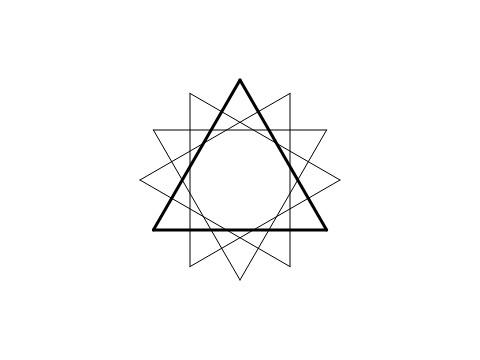
\includegraphics[width=.3\textwidth]{6-2-substar-12-4.png}}
  \end{center}
  Basically, one star is INSIDE another. Here are three stars. Find
  their MINIMAL (star with the least points) substars. 
  \begin{enumerate}
  \item $\stringstar{32}{8}$
  \item $\stringstar{60}{36}$
  \item $\stringstar{52}{32}$
  \end{enumerate}
  In each case, display your STAGE.  As a gesture of friendship, I give
  you my script:
  \begin{center}
    \includegraphics{substarScript.png}
  \end{center}
  Correctly using this script to produce a STAGE is sufficient for
  these answers.
  \begin{freeResponse}
    \begin{enumerate}
    \item
      \begin{center}
        \fbox{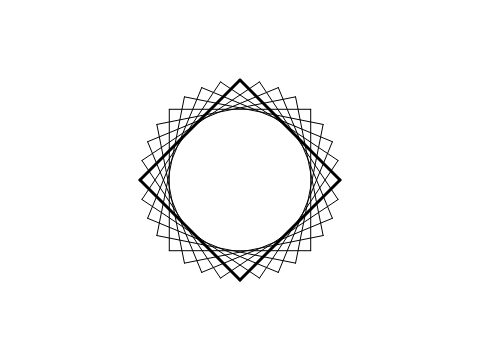
\includegraphics[width=.3\textwidth]{4-1-substar-32-8.png}}
      \end{center}
    \item
      \begin{center}
        \fbox{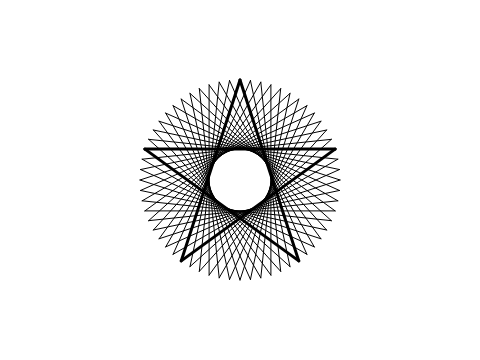
\includegraphics[width=.3\textwidth]{5-3-substar-60-36.png}}
      \end{center}
    \item
      \begin{center}
        \fbox{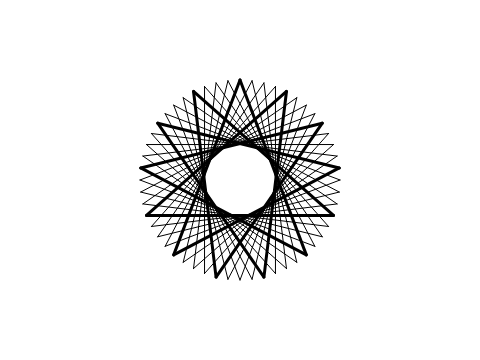
\includegraphics[width=.3\textwidth]{13-8-substar-52-32.png}}
      \end{center}
    \end{enumerate}
  \end{freeResponse}
\end{question}
\mynewpage





\begin{question}
  Substars have sub-symmetries.
  \begin{enumerate}
  \item Consider the star $\stringstar{12}{4}$ and
    \begin{itemize}
    \item $r$ a $30$ degree clockwise rotation with
    \item $f$ a flip across a vertical line through the center of the
      star.
    \end{itemize}
    Express the symmetries of the substar $\stringstar{3}{1}$ in the
    form $r^n f^m$.
  \item Consider the star $\stringstar{20}{5}$ and
    \begin{itemize}
    \item $r$ an $18$ degree clockwise rotation with
    \item $f$ a flip across a vertical line through the center of
      the star.
    \end{itemize}
    Express the symmetries of the substar $\stringstar{4}{1}$ in the
    form $r^n f^m$.
  \item Consider the star $\stringstar{21}{9}$ and
    \begin{itemize}
    \item $r$ a $(360/21)$ degree clockwise rotation with
    \item $f$ a flip across a vertical line through the center of the
      star.
    \end{itemize}
    Express the symmetries of the substar $\stringstar{7}{3}$ in the
    form $r^n f^m$.
  \end{enumerate}
  \begin{freeResponse}
  \item Here the symmetries are:
    \[
    \{e, r^4,r^8,f,r^4f,r^8f\}
    \]
  \item Here the symmetries are:
    \[
    \{e, r^5,r^{10},r^{15},f,r^5f,r^{10}f,r^{15}f\}
    \]
   \item Here the symmetries are:
    \[
    \{e, r^3,r^{6},r^{9},r^{12},r^{15},r^{18},f, r^3f,r^{6}f,r^{9}f,r^{12}f,r^{15}f,r^{18}f\}
    \]  
  \end{freeResponse}
\end{question}

\mynewpage


\begin{question} %% maximal star with substar sym.
Here's a more difficult question, and I'm asking you to think about
it. Here is a block:
\begin{center}
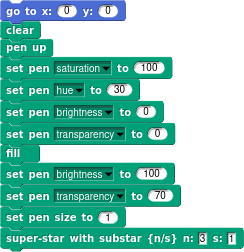
\includegraphics{substarCoolBlock.png}
\end{center}
What does it do? Well it draws a $\stringstar{n}{s}$ and then, it
draws the next $30$ stars that contain $\stringstar{n}{s}$ as a
substar. Now, this is kind of a mess, so what we've done is made:
\begin{itemize}
  \item The stars with the most symmetry, the most transparent.
  \item The stars with the least symmetry, the least transparent.
  \item The hue of the color to change between stars.
\end{itemize}
\begin{enumerate}
\item Describe the symmetry of this new figure.
\item Find and describe ``interesting'' features. Can you EXPLAIN
  THEM?
\end{enumerate}

\begin{freeResponse}
  \begin{enumerate}
  \item The symmetry of this figure is EXACTLY that of the
    triangle. This is because all of the symmetries must preserve THIS
    \begin{center}
      \fbox{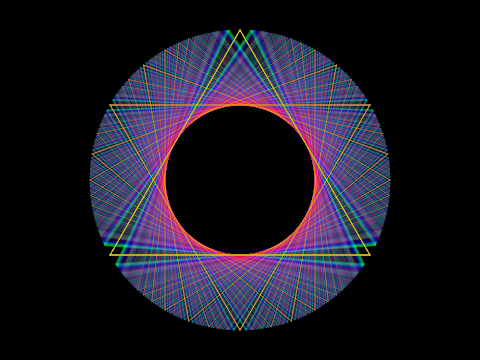
\includegraphics[width=.3\textwidth]{substarCoolStage.png}}
    \end{center}
    triangle.
  \item For me the most interesting feature is that that three points
    of the triangle are drastically different from the other three
    points (that would make) a star.

    This happens BECAUSE IT CAN. The symmetries do not need to be
    preserved near the points of the six pointed star that are not
    points of the regular triangle. Hence the picture is ``more
    messy'' there.
  \end{enumerate}
\end{freeResponse}


\end{question}
\end{document}
